\section{Auswertung}
\label{sec:Auswertung}

In drei Versuchsteilen werden die Intensitäten verschiedener Blenden in Abhängigkeit vom Abstand $d$ vom Intensitätsmaximum aufgenommen. 
Diese Werte sind in Tabelle \ref{tab:m} aufgetragen.
Der Dunkelstrom $I_0$ wird in jeder Messung wiederholt zu $I_0=\SI{1,2}{\nano\ampere}$ bestimmt und von den Werten in Tabelle \ref{tab:m} subtrahiert. 
Der Abstand zwischen Blende und Photodiode beträgt konstant $L=\SI{1,203}{\meter}$. 

Im Folgenden sollen verschiedene Spaltbreiten $b_i$ mit Hilfe des Beugungsbildes bestimmt werden. 
Über geometrische Überlegungen und Kleinwinkelnäherung kann der Beugungswinkel nach
\begin{equation}
	\varphi\approx \tan{\varphi}=\frac{|d-d_0|}{L}
	\label{eq:winkel}
\end{equation} 
genähert werden.

\subsection{Beugung am schmalen Einfachspalt}
\begin{figure}
\centering
	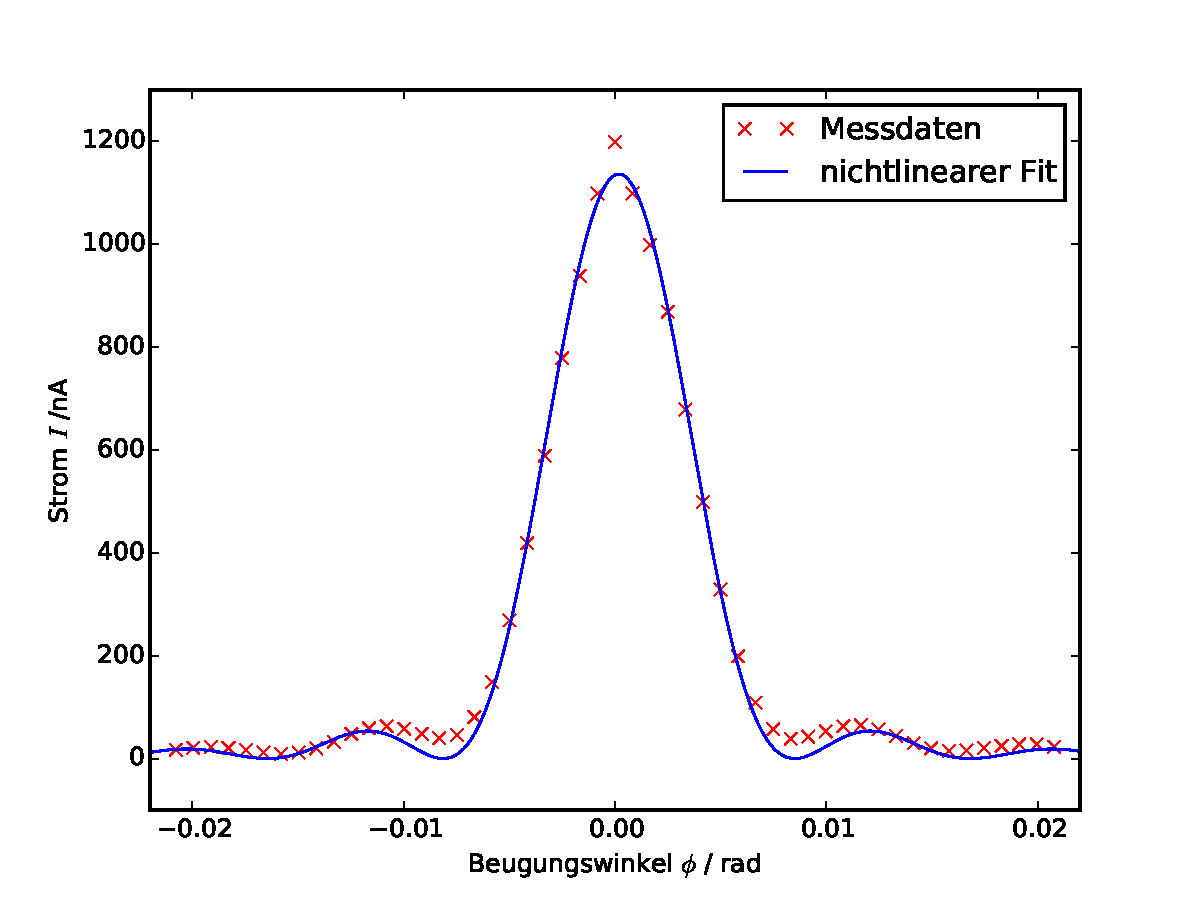
\includegraphics[width=0.8\textwidth]{Bilder/Messung1.pdf}
	\caption{Intensitätsverteilung bei Beugung am schmalen Einfachspalt.}
\label{fig:m1}
\end{figure}

Die Intensität $I_1={I_1}'-I_0$ wird in Abhängigkeit Beugungswinkel $\varphi$ wie in Abbildung \ref{fig:m1} aufgetragen. %, berechnet mit Gleichung\eqref{eq:winkel},
Eine nichtlineare Regression der Formel \eqref{eq:regress1} liefert die Amplitude \\$A_1=14,0\pm0,1$ ,
die Spaltbreite $b_1=({0,0761\pm0,0007}){\,\si{\milli\meter}}$ und eine Verschiebung der Kurve um $c_1=(-0.19\pm0.03)\cdot 10⁻³$. Laut Hersteller besitzt der Spalt eine Breite von $b_\mathup{1,h}=\SI{0.075}{\milli\meter}$. Ausgemessen mit einem Mikroskop ergibt sich $b_\mathup{1,m}=\SI{0.095}{\milli\meter}$.

\newpage
\subsection{Beugung am breiten Einfachspalt}

\begin{figure}
\centering
	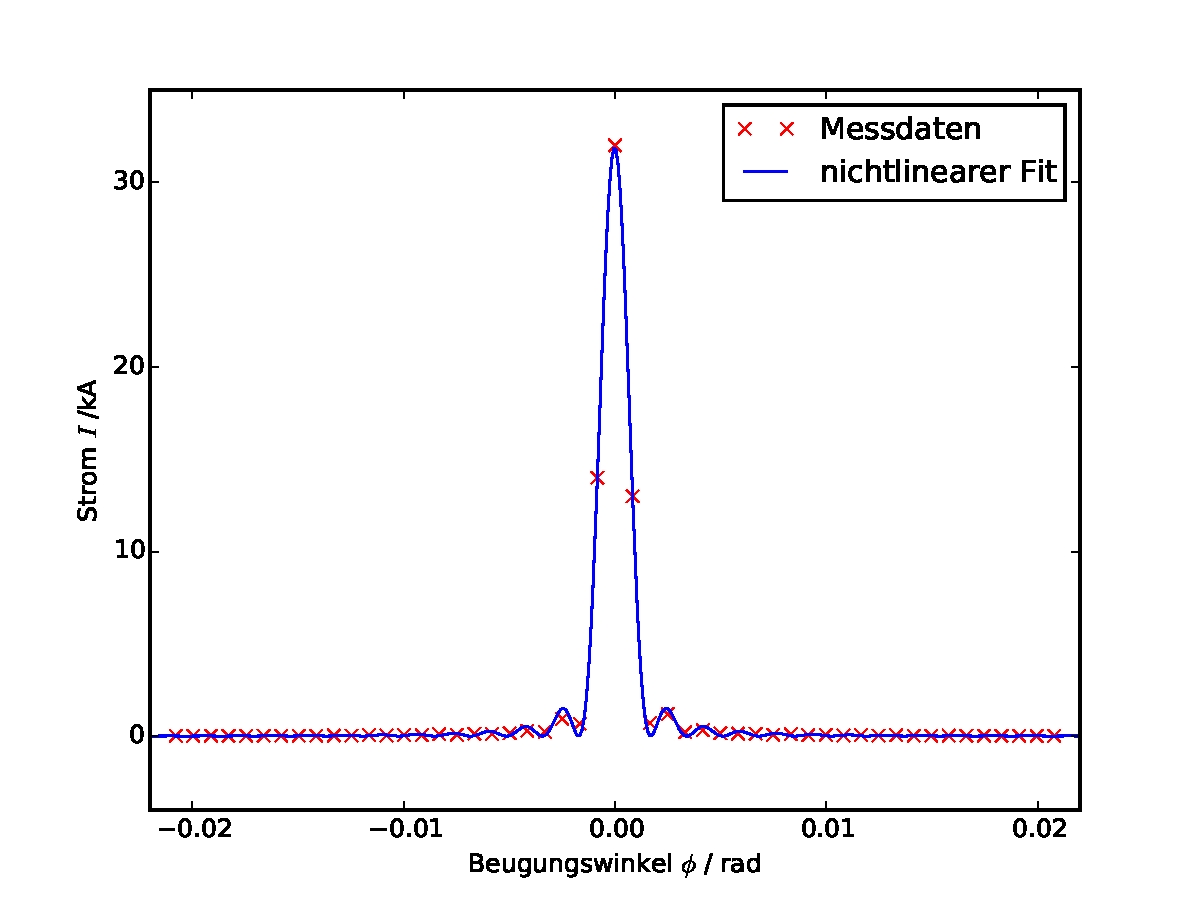
\includegraphics[width=0.8\textwidth]{Bilder/Messung2.pdf}
	\caption{Intensitätsverteilung bei Beugung am breiten Einfachspalt.}
\label{fig:m2}
\end{figure}

Erneut wird in Abbildung \ref{fig:m2} die Intensität $I$ in Abhängigkeit von $\varphi$ aufgetragen und eine nichtlineare Regression nach Gleichung \eqref{eq:regress1} ausgeführt. Es ergeben sich \\$A_2=15,21\pm0,08$, $b_2=(0,371\pm0,002)\,\si{\milli\meter}$ und $c_2=(20\pm 6)\cdot 10⁻⁶$. Die Messung mit dem Mikroskop ergibt $b_{\mathup{2,m}}=0,428\,\si{\milli\meter}$. Nach Herstellerangaben beläuft sich die Spaltbreite auf $b_\mathup{2,h}=\SI{0,4}{\milli\meter}$.

\subsection{Beugung am Doppelspalt}

Nebst Amplitude, Spaltbreite und Verschiebung der Kurve wird beim Doppelspalt der Abstand $g$ zwischen beiden Spalten bestimmt. Eine nichtlineare Regression nach \eqref{eq:regress2}, gezeigt in Abbildung \ref{fig:m3}, ergibt $A_3=18\pm1$, $b_3 =(0,099\pm0,007)\,\si{\milli\meter}$, \\$c_3=(-25\pm2)\cdot 10⁻⁶$ und $g_3=(0,490\pm0,006)\,\si{\milli\meter}$. Die Mikroskopmessung ergibt $b_\mathup{3,m}=\SI{0,143}{\milli\meter}$ und $g_\mathup{3,m}=0,524\,\si{\milli\meter}$. Die Hersteller geben $b_\mathup{3,h}=0,1\si{\milli\meter}$ und \\$g_\mathup{3,h}=0,4 \si{\milli\meter}$.

Aus Gleichung \eqref{eq:regress2} ist erkennbar, dass für ausgezeichnete x-Stellen die Cosinusquadrat-Verteilung maximal und normiert wird und damit  die Intensitätsverteilung \eqref{eq:regress1} der eines Einfachspalts gleicht.
Die Maxima des Kurvenverlaufes in Abbildung \ref{fig:m3} sind gesondert gekennzeichnet, die einhüllende Kurve ist ein Fit dieser Maxima mit der Funktionenklasse \eqref{eq:regress1}.
Damit ist die Beziehung zwischen Einzel- und Doppelspaltverteilung in Gleichung \eqref{eq:regress2} nachgewiesen.

\begin{figure}
\centering
	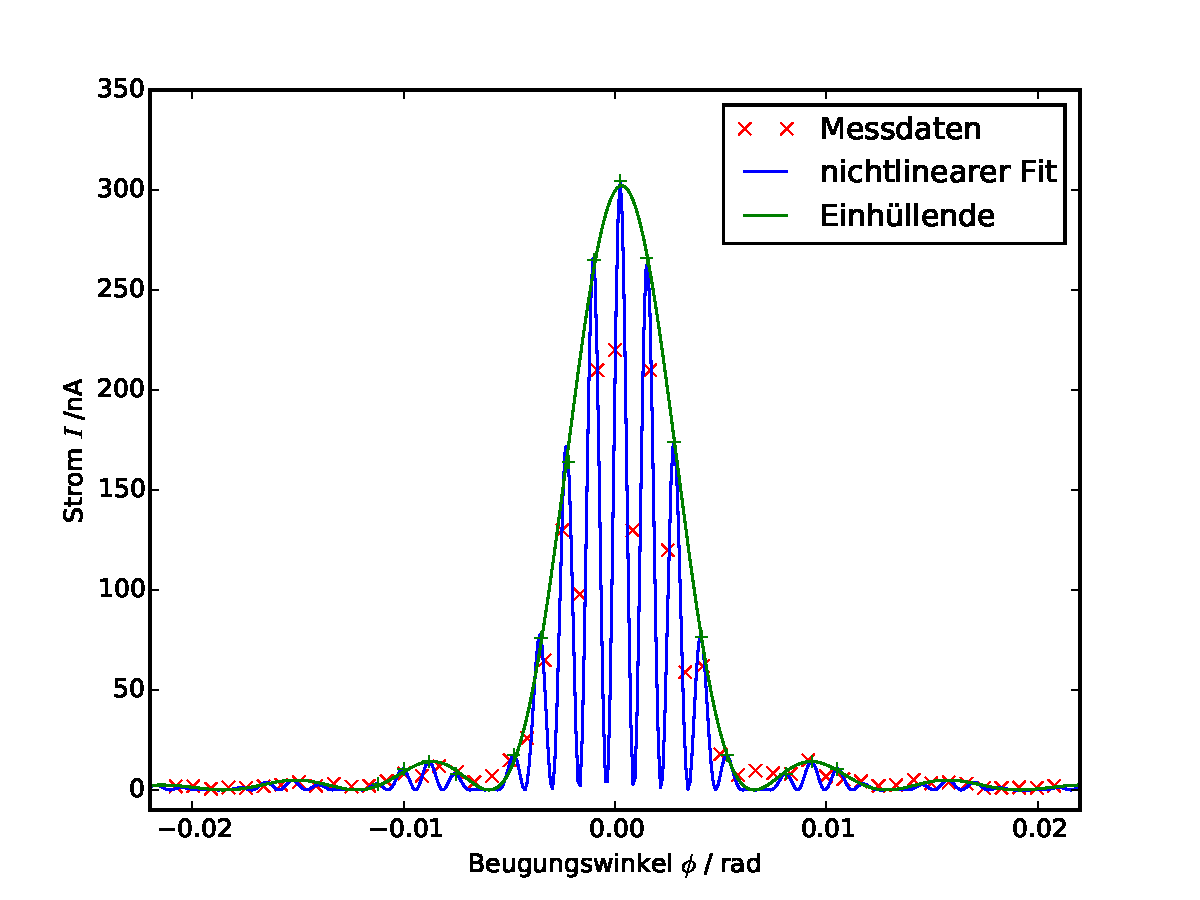
\includegraphics[width=0.9\textwidth]{Bilder/Messung3.pdf}
	\caption{Beugung am Doppelspalt.}
\label{fig:m3}
\end{figure}


\begin{table}
	\centering
	\sisetup{table-format=5.0}
	\begin{tabular}{S S S S}
	\toprule
	\multicolumn{1}{c}{Abstand} & \multicolumn{3}{c}{Intensität} \\
{$d/\:\si{\milli\meter}$} & {${I_1}'/\:\si{\nano\ampere}$} & {${I_2}'/\:\si{\nano\ampere}$} & {${I_3}'/\:\si{\nano\ampere}$}\\	
	\midrule
0 & 18 & 16 & 19\\
1 & 22 & 13 & 20\\
2 & 24 & 30 & 8\\
3 & 22 & 16 & 14\\
4 & 18 & 25 & 12\\
5 & 13 & 19 & 20\\
6 & 10 & 27 & 28\\
7 & 13 & 28 & 40\\
8 & 21 & 26 & 40\\
9 & 34 & 33 & 32\\
10& 49 & 30 & 18\\
11& 60 & 64 &23\\
12& 64 & 42 &46\\
13& 59& 68 & 84\\
14& 49 & 58 & 72\\
15& 41 & 110 &120\\
16& 47 & 82& 90\\
17& 82& 130&41\\
18& 150 & 130 &71\\
19& 270 & 160 & 150\\
20& 420 & 300 & 260\\
21& 590 & 230 & 650\\
22& 780 &940 &1300\\
23& 940&680&980\\
24&1100&14000&2100\\
25&1200&32000&2200\\
26&1100&13000&1300\\
27&1000&710&2100\\
28&870&1200&1200\\
29&680&220&590\\
30&500&320&620\\
31&330&160&180\\
32&200&140&76\\
33&110&130&98\\
34&58&78&85\\
35&40&110&82\\
36&44&52&150\\
37&54&72&69\\
38&64&34&55\\
39&66&58&44\\
40&58&29&22\\
41&45&46&25\\
42&31&30&52\\
43&21&25&34\\
44&16& 32& 39\\
45&17&21& 33\\
46&22&27& 12\\
47&26&14& 12\\
48&29&26& 14\\
49&29&12& 12\\
50&24&20& 22\\
	\bottomrule
\end{tabular}
	\caption{Messung der Intensitäten $I'_\mathup{i}$ in Abhängigkeit vom Abstand $d$.}
	\label{tab:m}
\end{table}

